\documentclass[12pt,a4paper]{article}
% \usepackage[english]{babel}
% \usepackage[utf8x]{inputenc}

\usepackage{graphicx} % Required for inserting images.
\usepackage[margin=25mm]{geometry}
\parskip 4.2pt  % Sets spacing between paragraphs.
% \renewcommand{\baselinestretch}{1.5}  % Uncomment for 1.5 spacing between lines.
\parindent 8.4pt  % Sets leading space for paragraphs.
\usepackage[font=sf]{caption} % Changes font of captions.

\usepackage{amsmath}
\usepackage{amsfonts}
\usepackage{amssymb}
\usepackage{siunitx}
\usepackage{verbatim}
\usepackage{hyperref} % Required for inserting clickable links.
\usepackage{natbib} % Required for APA-style citations.


\title{Do cryptocurrencies extend the mean-variance frontier of an equity investor?}
\author{Sander Naerum, Thomas Pietsch and Ziga Jagodnik}

\begin{document}
\maketitle

\begin{abstract}
In this project we will investigate if cryptocurrencies extend the mean-variance frontier of an equity investor. 
By using an industry portfolio dataset consisting of 12 different industries collected from Kenneth French website 
combined with “” cryptocurrency index, we extract the mean-variance frontier. We show that adding cryptocurrencies to 
the mean-variance frontier do not have a significant impact.  
\end{abstract}

\section{Introduction}\label{sec:intro}
The mean-variance frontier is a mathematical framework for building portfolios that aim to maximize expected returns 
while controlling a set level of risk. This concept extends diversification in investing, highlighting that owning 
diverse financial assets is less risky than focusing on a single asset class. The key idea is that an asset's risk and 
return should be evaluated in the context of its contribution to the overall risk and return of a diversified portfolio. 
Historical asset price variance is used as a proxy for estimating future risk in the mean-variance frontier.

In the evolving landscape of financial assets, the integration of cryptocurrencies adds a new dimension to portfolio 
construction. Cryptocurrencies, such as Bitcoin and Ethereum, bring unique characteristics and opportunities to the mix. 
Therefore, it is interesting to explore if this new universe of assets can enhance portfolio diversification. 

\section{Methodology}\label{sec:methods}
\subsection{Assumptions under the MPT}
\begin{itemize}
\item Investors prefer higher returns for a given level of risk or aim to minimize risk for a given level of returns.
\item The degree of risk aversion varies among investors.
\item Investors have complete information about expected returns, variances, and covariances for all assets.
\item Investment returns are assumed to follow a normal distribution.
\item Only returns, variances, and covariances are needed to calculate the optimal portfolio.
\item No transaction costs or taxes.
\item We assume the risk-free rate to be equal to the current 3m Treasury yield of "", and all investors can borrow and lend at this rate. 
\end{itemize}
The mean-variance analysis is used to identify optimal/efficient portfolios.

\subsection{Return calculations}
The data downloaded from Kenneth French's website is already calculated as simple returns, however, in this paper we will use the log returns of the assets. To convert the simple returns to log, we use the following formula: 
$$r_i = ln(1+r_i)$$

\noindent For the data on the crypto prices downloaded from yahoo finance we use the following formula to obtain the log returns: 
$$r_i = ln(\frac{P_t}{P_t-1})$$

\section{Data}\label{sec:result}
\textbf{Equity data:} Kenneth French website, 12 industry portfolios. 

\noindent\textbf{Crypto's:} Imported the 5 largest crypto currencies based on market cap, source: Yahoo Finance.  

\subsection{Frontier construction}
The Sharpe-ratio of a security: 
$$\textit{Sharpe Ratio} = \frac{E[r_i] - r_f}{\sigma(r_i)}$$

\noindent The variance-covariance matrix of assets: 
\[
\text{Covariance Matrix:}
\begin{bmatrix}
    \sigma_{1}^2 & \sigma_{12} & \sigma_{13} \\
    \sigma_{12} & \sigma_{2}^2 & \sigma_{23} \\
    \sigma_{13} & \sigma_{23} & \sigma_{3}^2 \\
\end{bmatrix}
\]

\section{Discussion}\label{sec:discussion}

Blah

\subsection{Limitations}\label{sec:limitations}

Blah blah

\subsection{Figures}\label{sec:future}

\begin{figure}
    \centering
    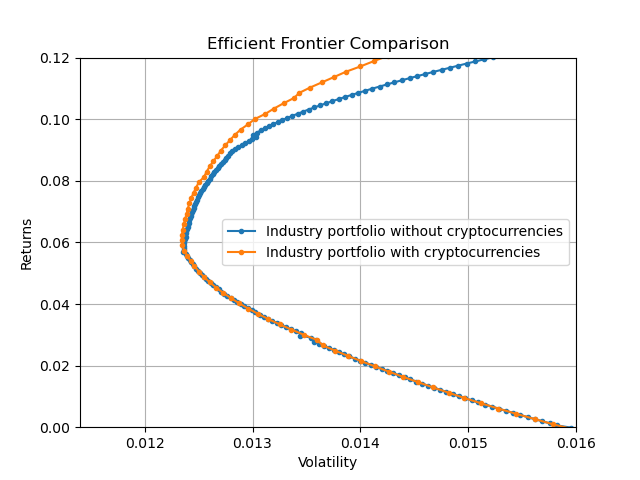
\includegraphics[width=1\linewidth]{figures/figure1.png}
    \caption{Comparing the two mean-variance frontiers}
    \label{fig:enter-label}
\end{figure}


\begin{figure}[htbp!]
\begin{center}
\includegraphics[width=0.5\columnwidth]{venn_discoveries.pdf}
\end{center}
\caption{Yes, put a few words or sentences here explaining what is in the figure.}
\label{fig:venn}
\end{figure}

\bibliographystyle{apalike}
\bibliography{example}

\end{document}
